\section{Validierung}\label{sec:Validierung}
Das Ziel der Validierung ist es, abzuklären, ob die gewählte Ansteuerung und der Brushless-Gleichstrommotor (BLDC) die verlangten Anforderungen erfüllen. Ausserdem wird das Steuerverhalten auf verschiedene Faktoren wie zum Beispiel Spannungsabfall, Laständerung und Steuerkennlinie untersucht.
Im ersten Unterkapitel wird die Versuchsanordnung gezeigt, welche bei allen Versuchen gleich blieb. Die darauffolgenden Unterkapitel beschreiben die jeweilige Messung und die Auswertung des Versuches. Am Schluss des Kapitels werden dann die Erkenntnisse der Versuche kurz zusammengefasst.
Alle Messdaten sind im Anhang \ref{appsec:Messdaten} ersichtlich.


\subsection{Versuchsaufbau}\label{subsec:Versuchsaufbau}
Für den Versuchsaufbau wurde der BLDC mit einer asynchronen Maschine (ASM) gekoppelt, welche über einen Frequenzumrichter angesteuert wird und netzspeisefähig ist. Die ASM simuliert bei den nachfolgenden Versuchen die Last.


\begin{figure}[H]
	\begin{center}
		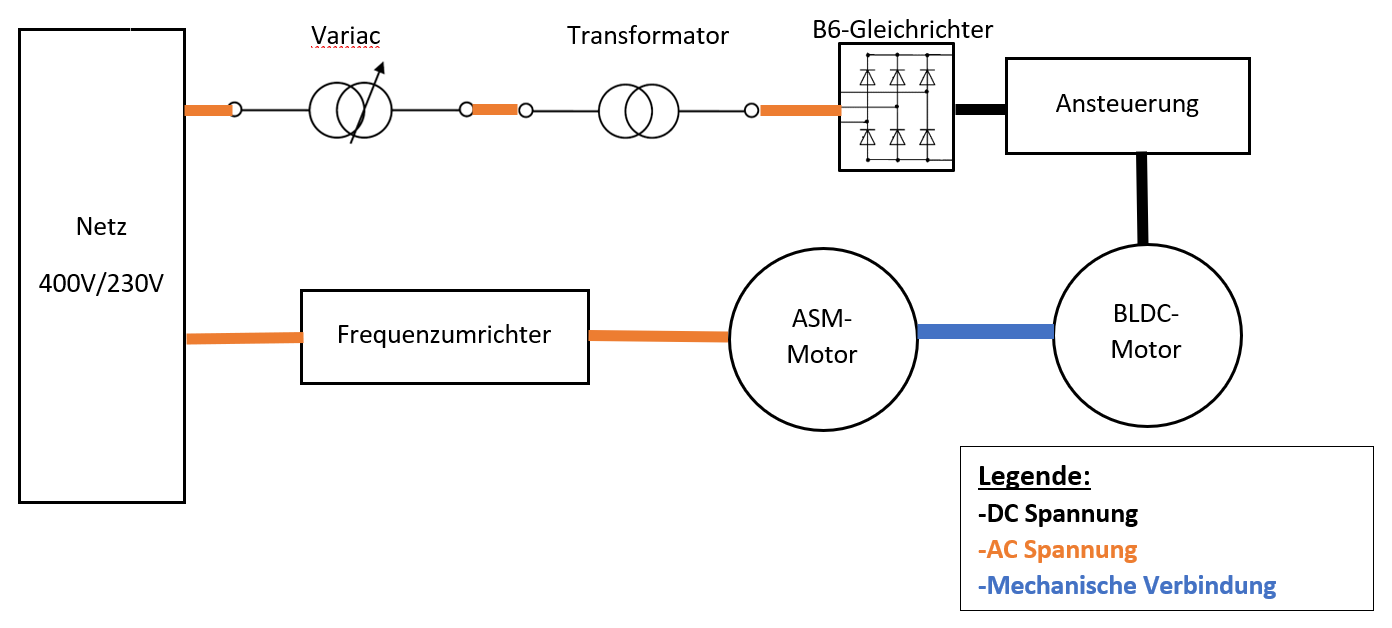
\includegraphics[height=70mm]{Versuchsaufbau/Schema.png}
		\caption{Schema Versuchsaufbau}
		\label{fig:Schema}
	\end{center}
\end{figure}

Um die verschiedene Versuche auszuwerten, wurde je nach Versuch verschiedene Gössen gemessen.
Die \textbf{Spannung} und der \textbf{Strom} wurde zwischen der Ansteuerung und dem B6-Gleichrichter gemessen. Die \textbf{Drehzahl} wurde mithilfe eines Oszillator ausgewertet. Dabei wurde dieser direkt an einem Hallsensor angehängt, welcher vier Impulse pro Umdrehung generiert. Die \textbf{Leistung} wurde mithilfe eines Power-Analyzers zwischen der ASM und dem Frequenzumrichter gemessen. Der \textbf{Drehmoment-Sollwert} wurde digital mit einem Mikrocontroller erzeugt und auf die Ansteuerung gegeben. Die \textbf{Motor-} und \textbf{Controller-Temperatur} wurden direkt am Computer ausgelesen, welcher an der Ansteuerung angeschlossen ist.\\

Wie auf dem Schema auf der Abbildung \ref{fig:Schema} ersichtlich, erfolgt die Energieversorgung durch das Netz und wird auf einen Variac (Abbildung \ref{fig:Variac}) geführt, welcher nachfolgend abgebildet ist.

\begin{figure}[H]
	\begin{center}
		\includegraphics[height=80mm]{Versuchsaufbau/DSC00555.jpg}
		\caption[Variac Versuchsaufbau]{Variac Versuchsaufbau}
		\label{fig:Variac}
	\end{center}
\end{figure}

Die Einspeisung des Variacs erfolgte durch eine CEE-63A Steckdose und ist auf der Abbildung nicht ersichtlich. Die Regulierung des Variacs erfolgt mittels drehen am kleinen schwarzen \glqq Steuerrad\grqq \space (unten links) und gibt bei Dreieckschaltung eine Ausgangsspannung zwischen 0-290V und einen maximalen Strom von 50A. Da unser Motor lediglich eine Betriebsspannung von 96V und im Nennbetrieb einen Strom von deutlich über 100A benötigt, wird ein Transformator nachgeschaltet (Abbildung \ref{fig:Trafo}). Der Anschluss erfolgte Primärseitig und Sekundärseitig in Dreieckschaltung und hat einen sekundären Maximalstrom von $95A_{AC}$ bei $127V_{AC}$. Die Gleichrichtung erfolgt mittels einer B6-Brücke, welche während diesem Projekt selber gebaut wurde. Der Aufbau ist in Abbildung \ref{fig:B6} ersichtlich.

\begin{figure}[H]
	\centering
	\begin{minipage}[H]{.4\linewidth} % [b] => Ausrichtung an \caption
		\centering
		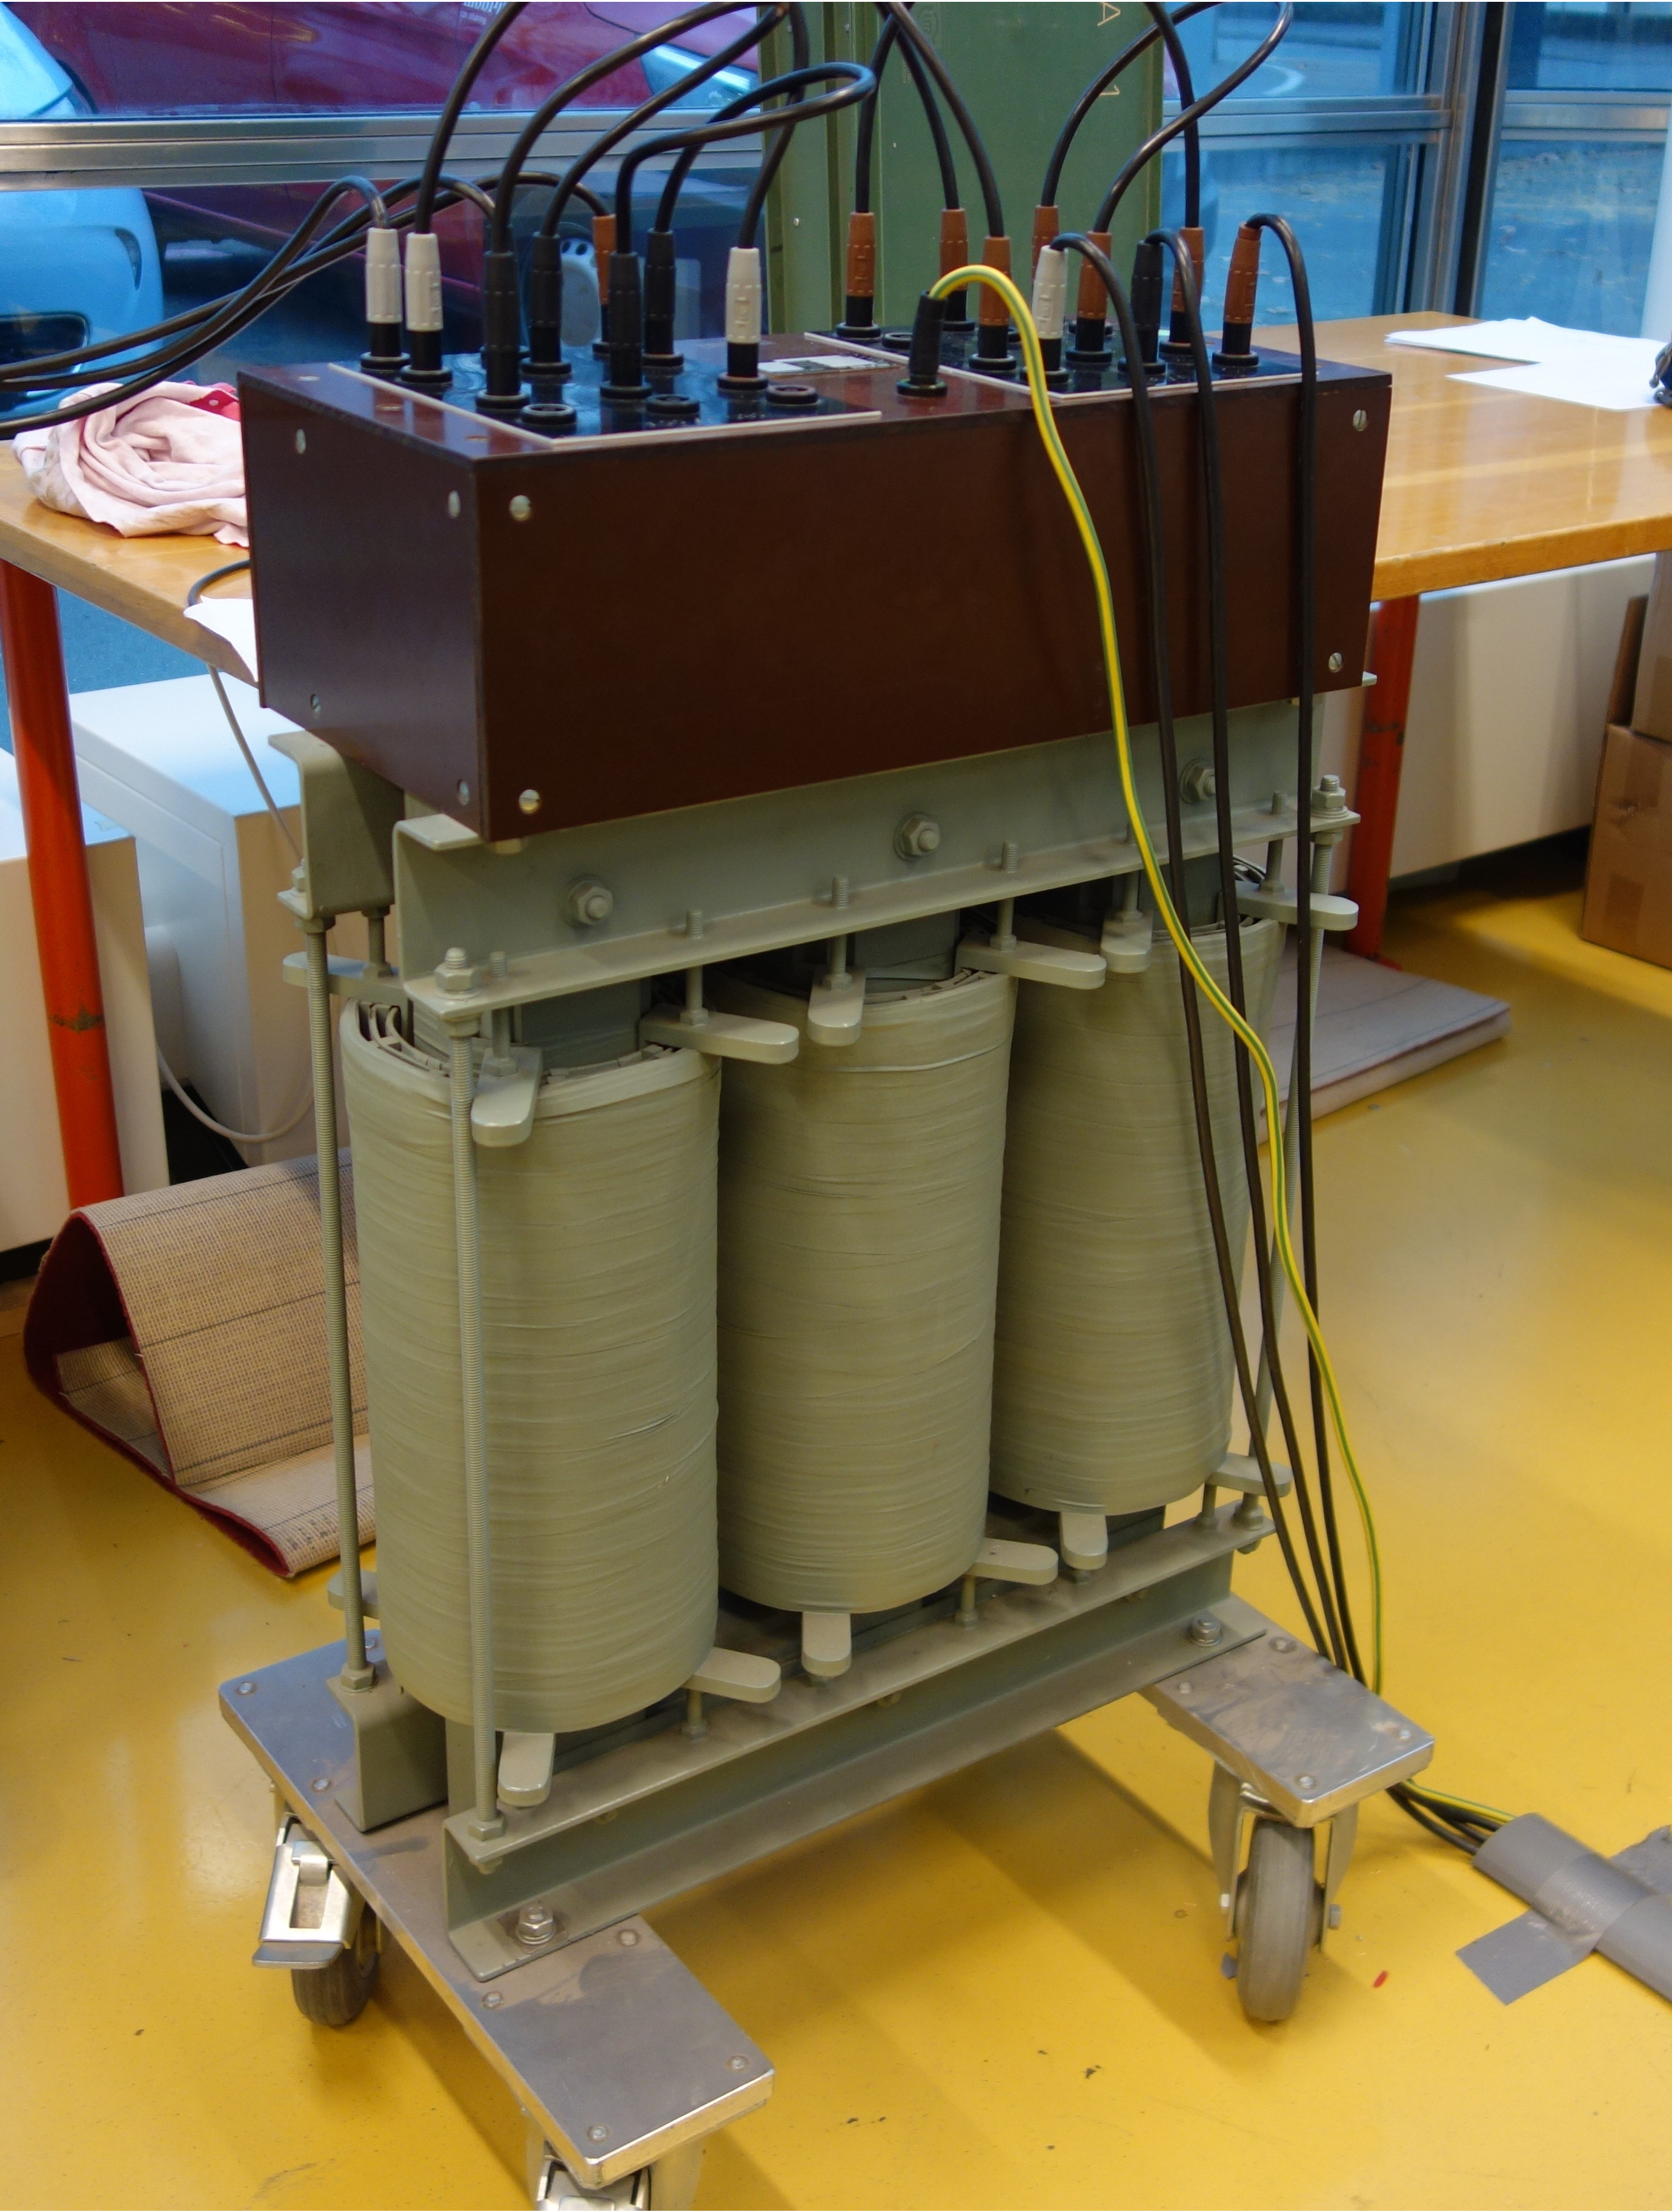
\includegraphics[width=\linewidth]{Versuchsaufbau/DSC00556.jpg}
		\caption[Transformator Versuchsaufbau]{Transformator}
		\label{fig:Trafo}
	\end{minipage}
	\ % Abstand zwischen Bilder
	\begin{minipage}[H]{.4\linewidth} % [b] => Ausrichtung an \caption
		\centering
		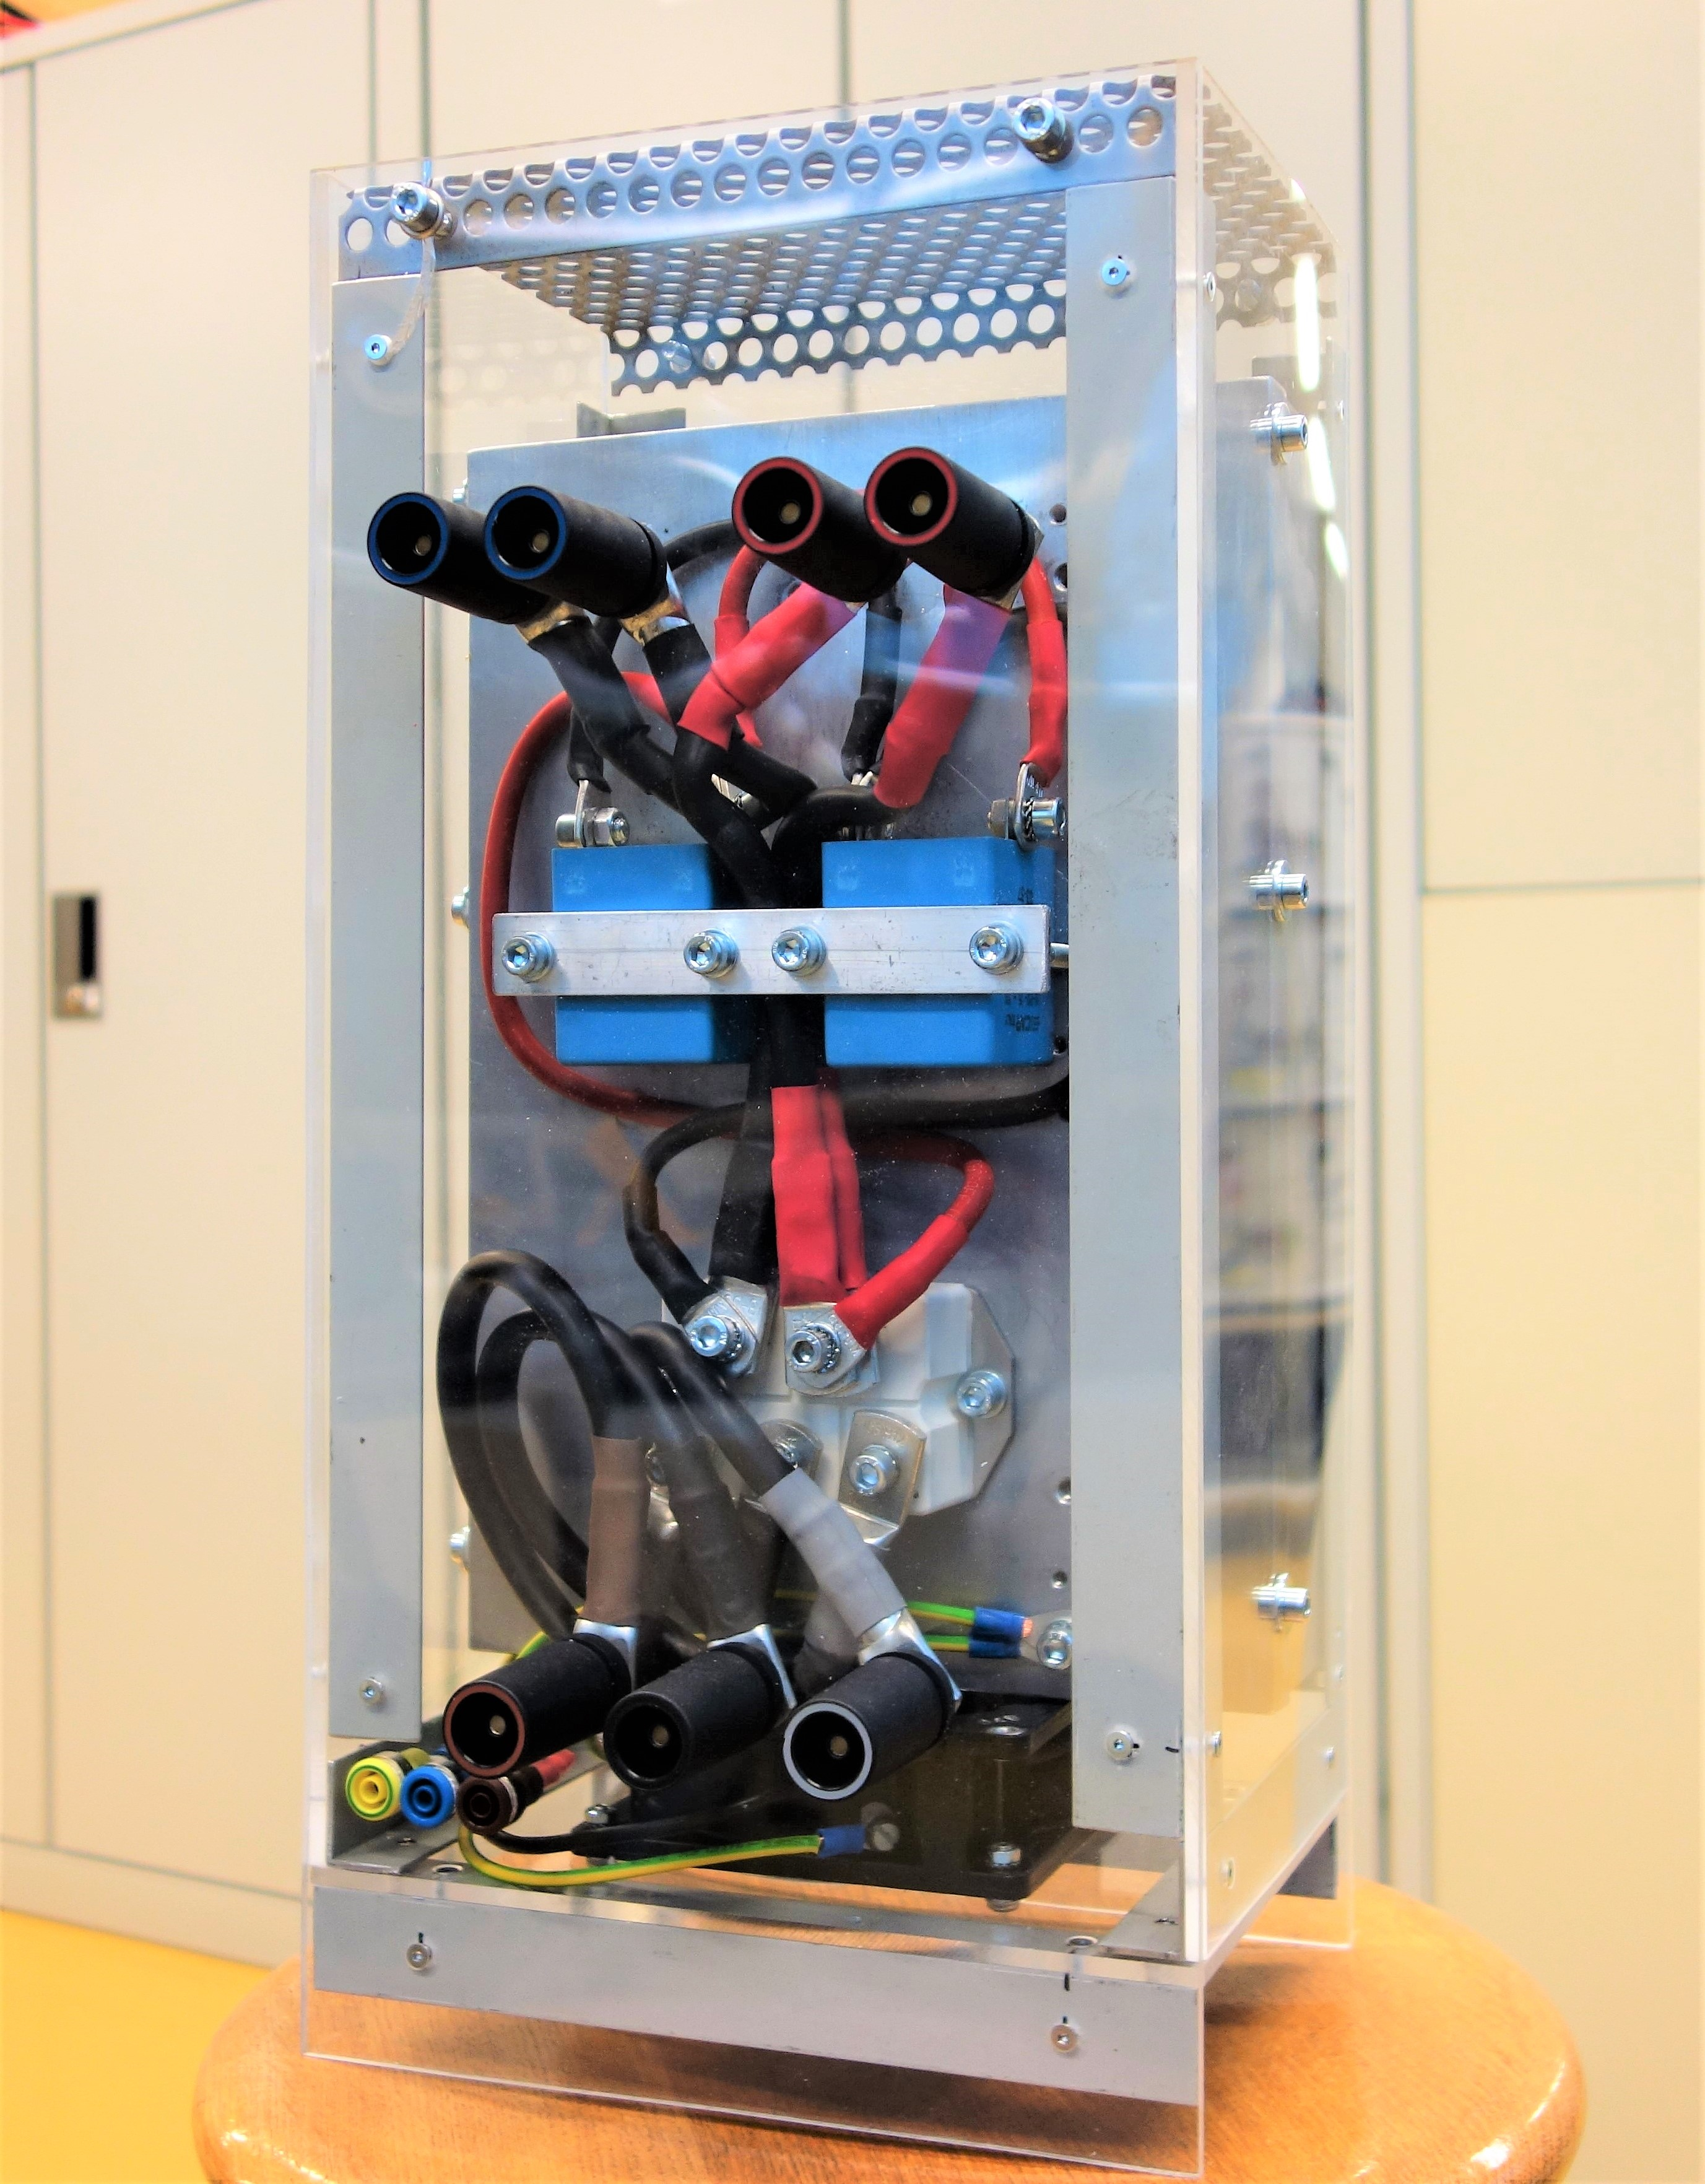
\includegraphics[width=\linewidth]{Versuchsaufbau/DSC00547(2).jpg}
		\caption[B6 Gleichrichter]{B6 Gleichrichter}
		\label{fig:B6}
	\end{minipage}
\end{figure}

Die AC-Einspeisung der B6-Brücke erfolgt mittels den drei Klemmen (Braun, Schwarz, Grau) im unteren Bereich. Diese werden auf den eigentlichen Diodengleichrichter (Weiss) und zwei Stützkondensatoren (Blau) geführt.Gemäss der Formel \ref{eq:B6-Id} ergibt sich somit einen maximalen Zwischenkreisstrom auf der DC Seite von $I_{DC}=\frac{95A}{0.8165} =\underline{116.35A}$.
Dieser erhöhte Strom, wird DC-Seitig durch jeweils zwei Hin-, und Rückleiter (Blau und Rot) auf die Motorenansteuerung geführt.\\
Die zwei Elektrolytkondensatoren (Elkos), welche in der Abbildung \ref{fig:Controller} ganz links ersichtlich sind, dienen zur Glättung der Gleichstromversorgung bei hohen Belastungen. Der Controller ist rechts im Bild ersichtlich, dazwischen befindet sich noch ein DC-Relais, welches vom Controller angesteuert wird und die DC-Speissung unterbrechen kann.

\begin{figure}[H]
	\begin{center}
		\includegraphics[height=80mm]{Versuchsaufbau/DSC00581.jpg}
		\caption[Controller]{Controller}
		\label{fig:Controller}
	\end{center}
\end{figure}

Tritt ein Fehlerfall auf, kann der Controller mithilfe des DC-Relais die Stromversorgung unterbrechen. Etwas schwer auf der Abbildung zu erkennen sind die Kontakte auf dem Controller. Dieser besitzt eine Sicherung direkt nach der Einspeisung des +Pols. Weiter ist ein geflechteter Kabelbaum ersichtlich (welcher alle Kabel zur Ansteuerung des Controllers beinhaltet) und die farbigen Anschlusskabel des Motors auf der rechten Seite.\\
Aus Sicherheitsgründen wurden alle blanken Elemente mit Klebestreifen isoliert und der Controller, die Elkos und das DC-Relais mit einer Kiste abgedeckt.

Der Drehmoment-Sollwert für die Ansteuerung wurde mit einem Arduino-Controller erzeugt. Dabei wurde der PWM-Ausgang mithilfe eines RC-Tiefpasses in ein Spannungssignal gewandelt. Mithilfe eines Schmitt-Triggers konnte zudem die Drehzahl des Motors gemessen und geregelt werden. Auf der Abbildung \ref{fig:Mikrocontroller} ist das Arduino-Board ersichtlich. Darauf aufgebaut ist eine Experimentierplatine mit drei Taster (rechts) um den Sollwert einzustellen, einem Schmitt-Trigger (mitte) und dem RC-Tiefpass (links).

\begin{figure}[H]
	\begin{center}
		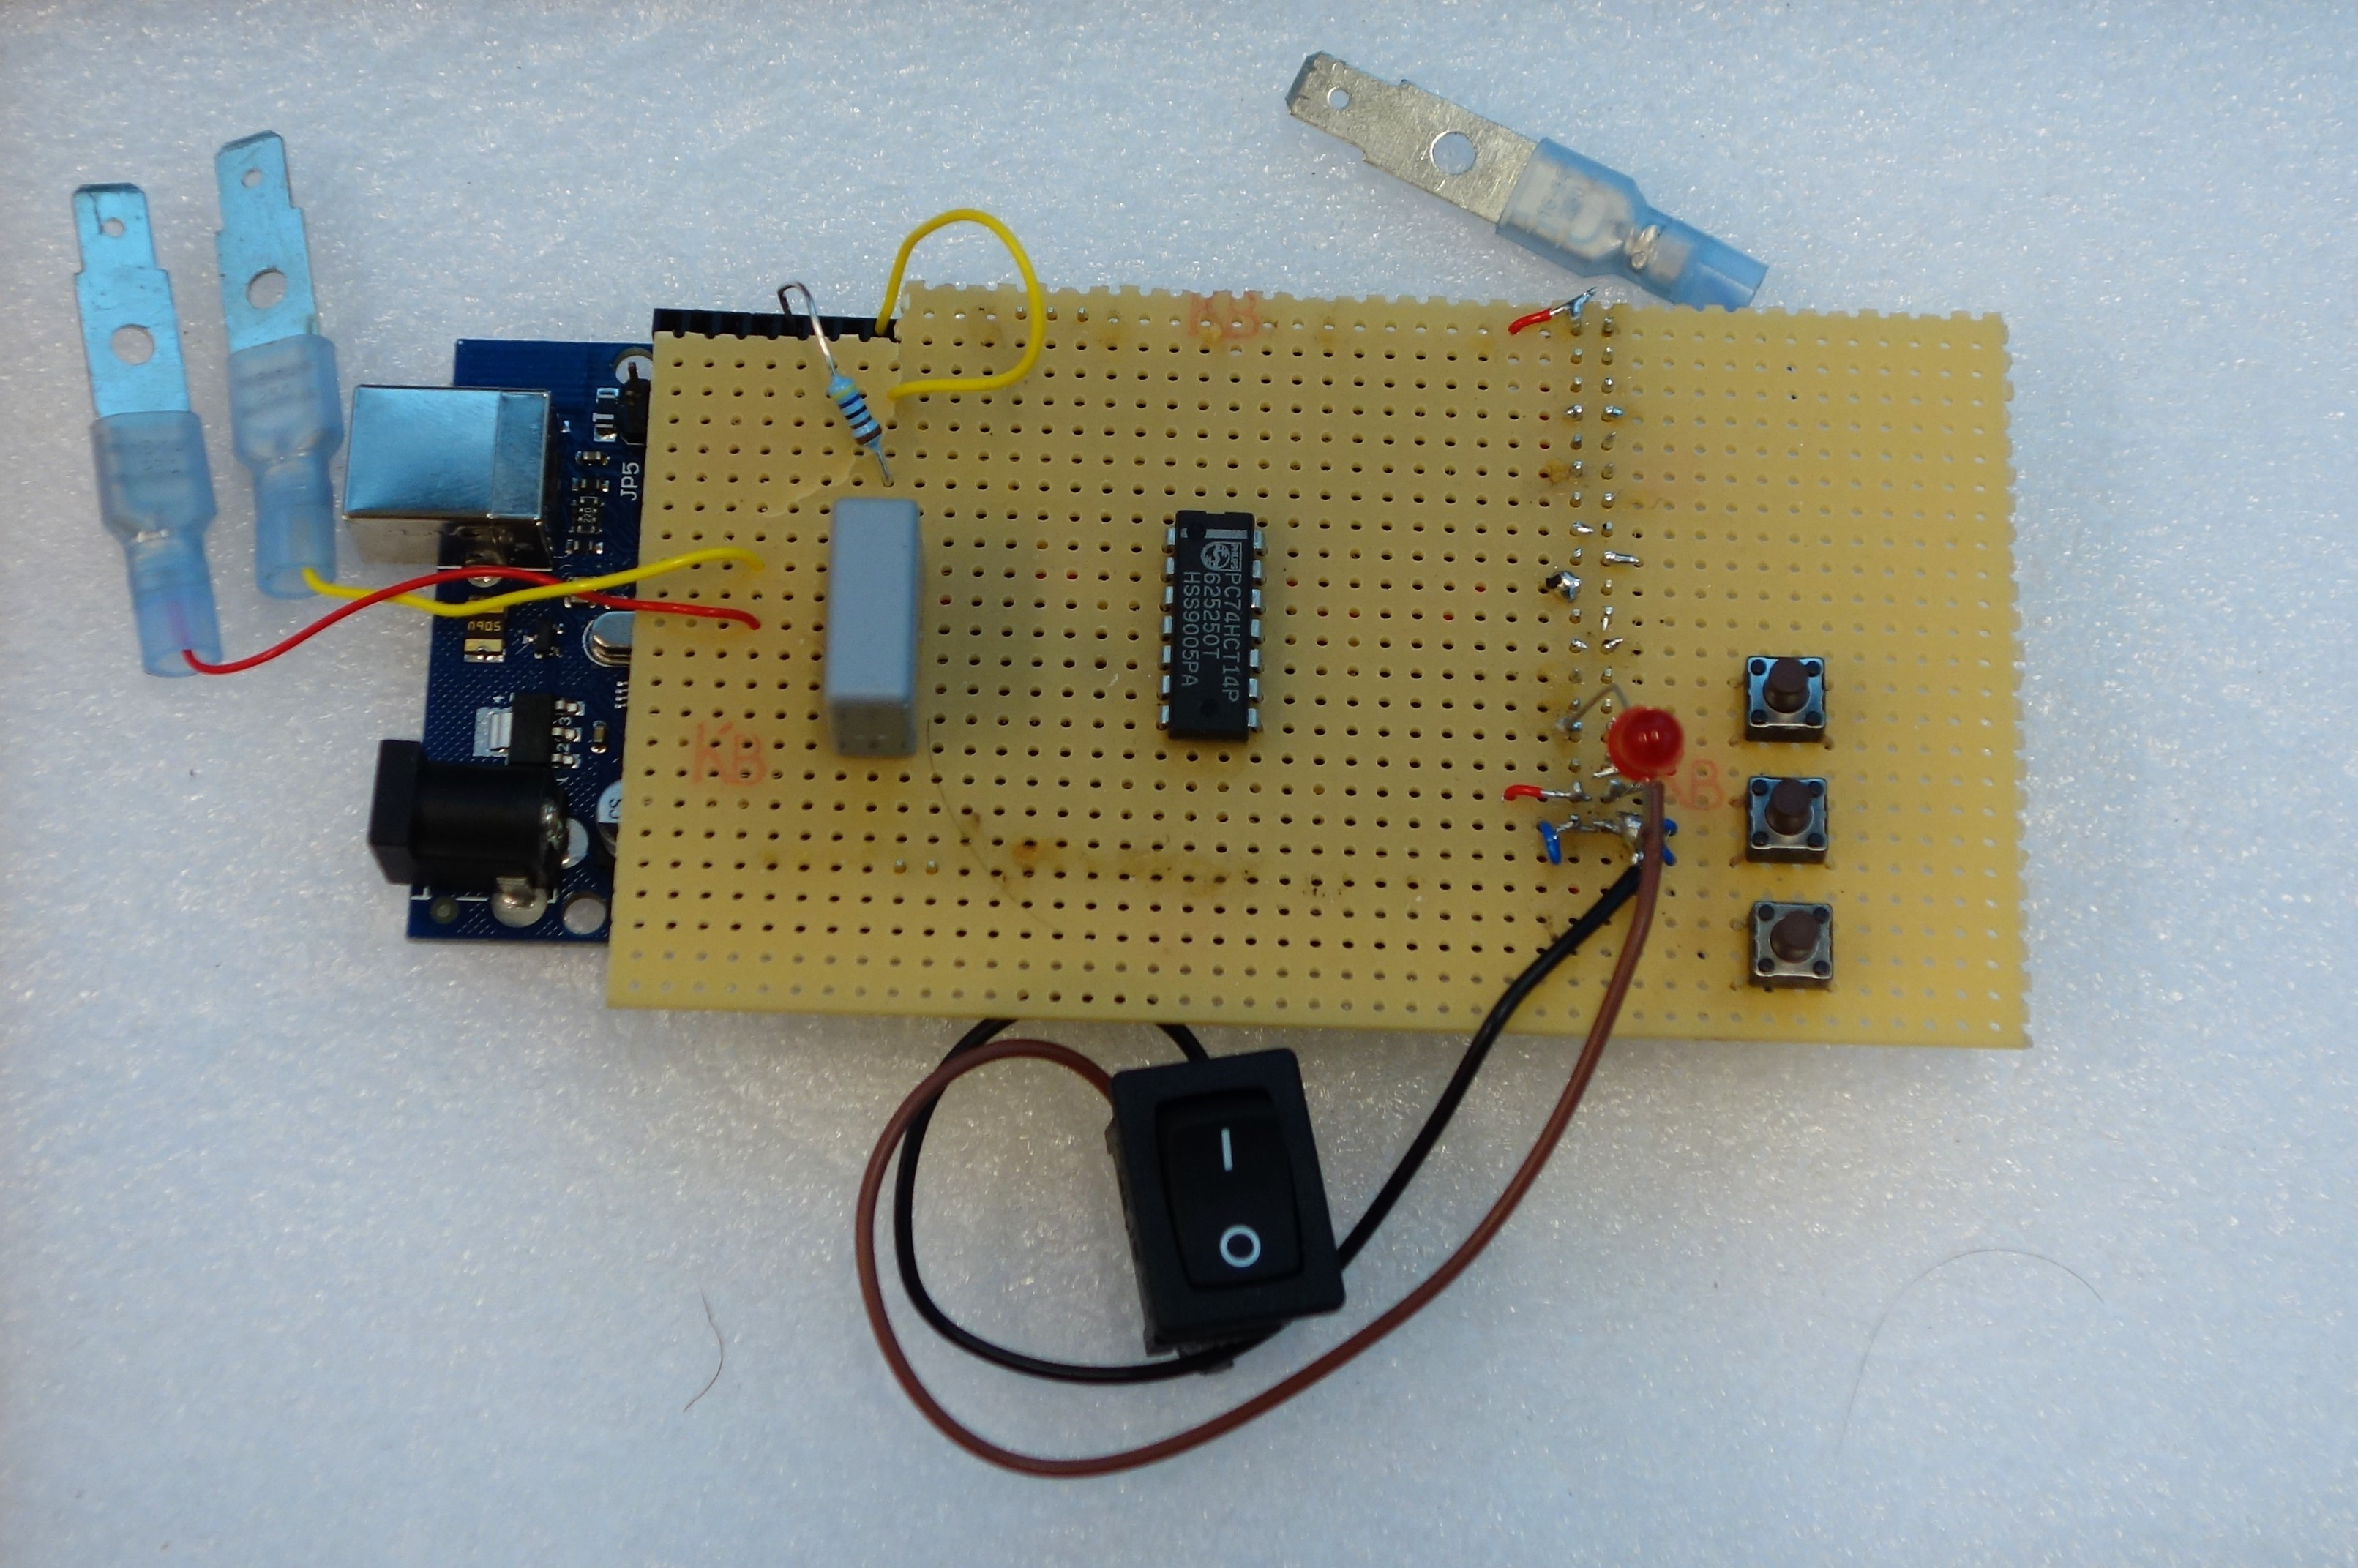
\includegraphics[height=60mm]{Versuchsaufbau/DSC00559.jpg}
		\caption[Controller]{Controller mit Experimentierplatine}
		\label{fig:Mikrocontroller}
	\end{center}
\end{figure}

Wie anfänglich bereits beschrieben wurde, wurde der verwendete BLDC Motor mit einer ASM gekoppelt. Die Anordnung ist in Abbildung \ref{fig:MotorenLueftung} links dargestellt. Damit diese zwei Maschinen überhaupt miteinander gekoppelt werden konnten, musste einerseits die Welle des BLDC Motors (links) auf das Niveau der ASM (rechts) angehoben werden und andererseits mussten einige Anpassungen an der Kupplung getätigt werden. Da der DC-Motor über eine Welle mit Zollmass verfügt, musste die Öffnung einer Kupplung ausgebohrt werden. Weiter verfügt die ASM über keine Nut, weshalb die andere Seite der Kupplung zur Befestigung mit einem Gewinde versehen werden musste. Die Befestigung erfolgt mittels zwei M8-Schraube, welche auf die Welle drücken. Für den Berührungsschutz sorgt eine Plexiglasscheibe über der mechanischen Verbindung.


\begin{figure}[H]
	\begin{center}
		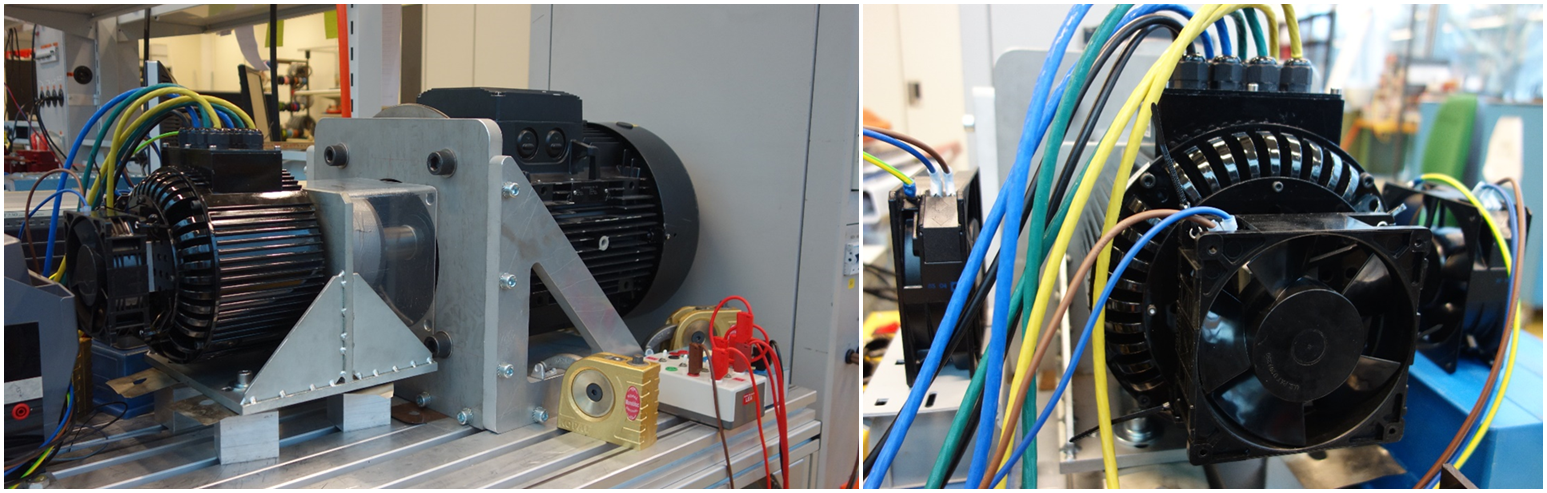
\includegraphics[width=\linewidth]{Versuchsaufbau/MotorLueft.png}
		\caption[Motoren Aufbau und Motorenlüftung]{Motoren Aufbau (links) und Motorenlüftung (rechts)}
		\label{fig:MotorenLueftung}
	\end{center}
\end{figure}

Leider weisst der verwendete Motor eine schlechte Eigenkühlung auf, wodurch zusätzliche Ventilatoren notwendig sind. In unseren Temperaturtests \ref{subsec:Temperatur} wurden zur Kühlung externe 110mm Ventilatoren verwendet. In Abbildung \ref{fig:MotorenLueftung} Grafik rechts, wurde die Anordnung seitlich und hinter dem Motor gewählt.


Damit überhaupt Leistungsversuche möglich sind, muss neben dem Gleichstrommotor auch die ASM angesteuert werden. Hierbei diente ein Frequenzumrichter (Abbildung \ref{fig:Frequenzumformer}) mit integrierter Netzschaltung. Die Versorgung erfolgt mittels einem CEE-32A Stecker und ist dementsprechend mit 32A abgesichert.

\begin{figure}[H]
	\centering
	\begin{minipage}[h]{.4\linewidth} % [b] => Ausrichtung an \caption
		\centering
		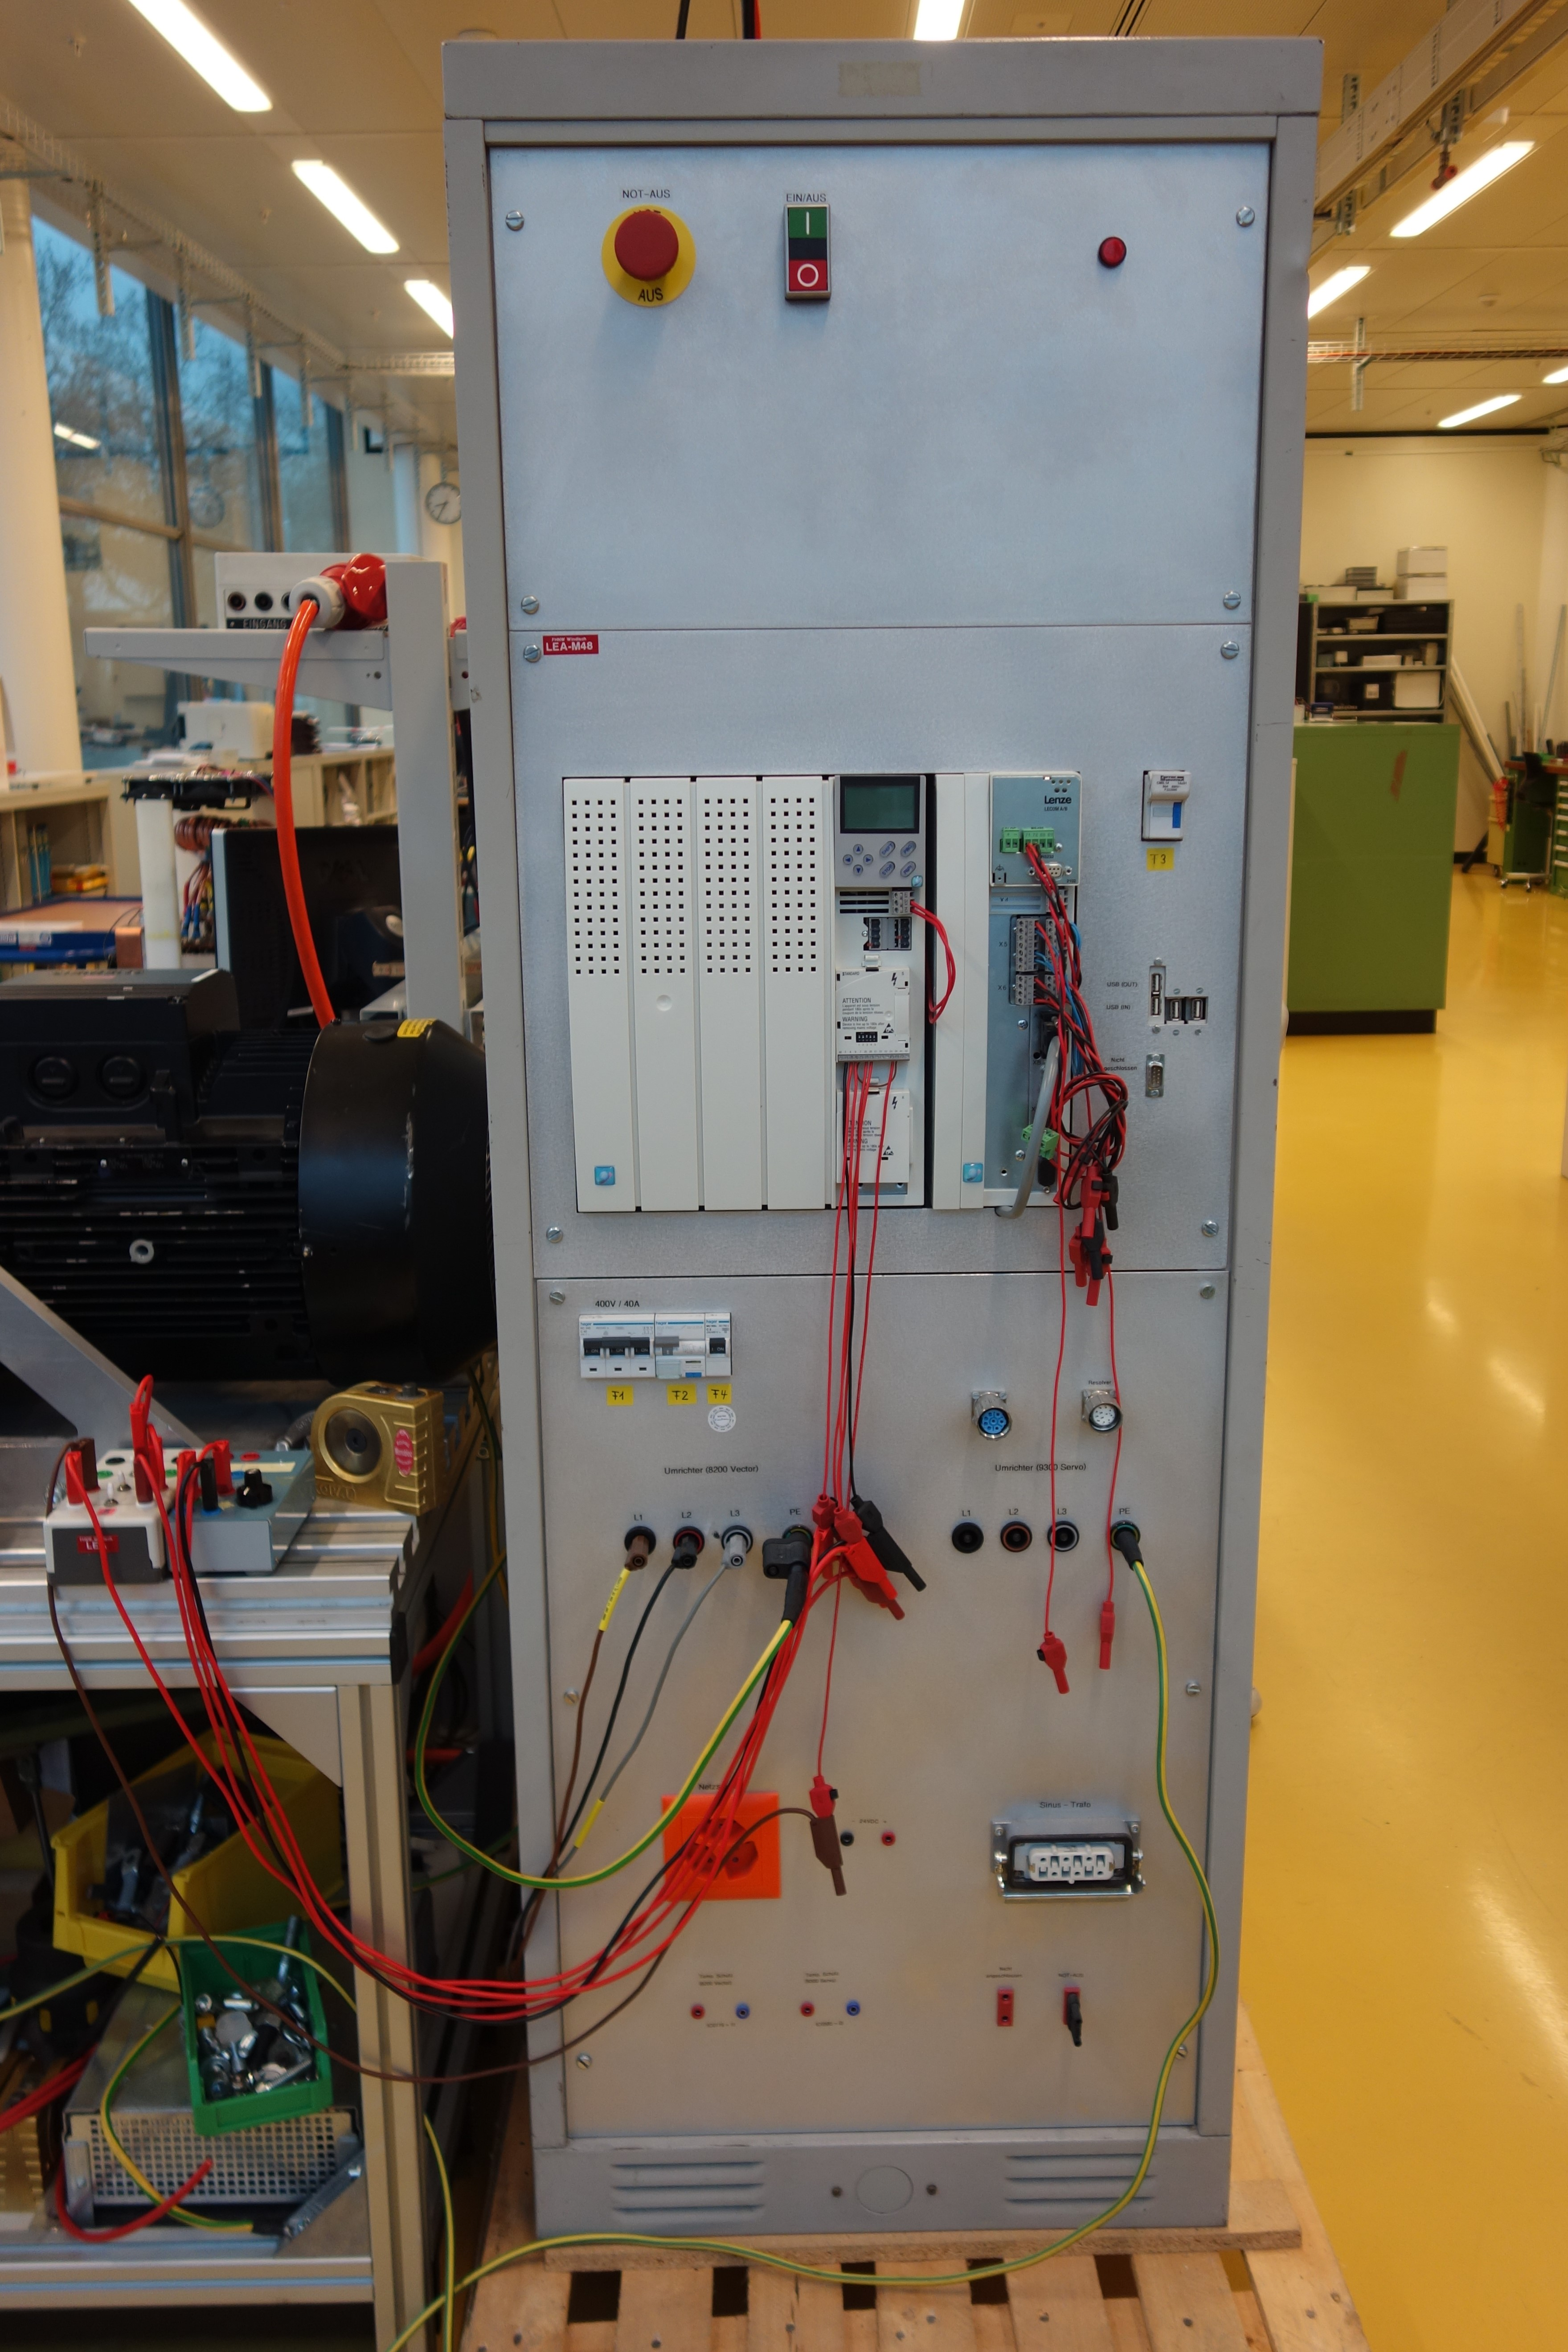
\includegraphics[height=100mm]{Versuchsaufbau/DSC00575.jpg}
		\caption[Frequenzumformer]{Frequenzumformer}
		\label{fig:Frequenzumformer}
	\end{minipage}
	\quad % Abstand zwischen Bilder
	\begin{minipage}[h]{.4\linewidth} % [b] => Ausrichtung an \caption
		\centering
		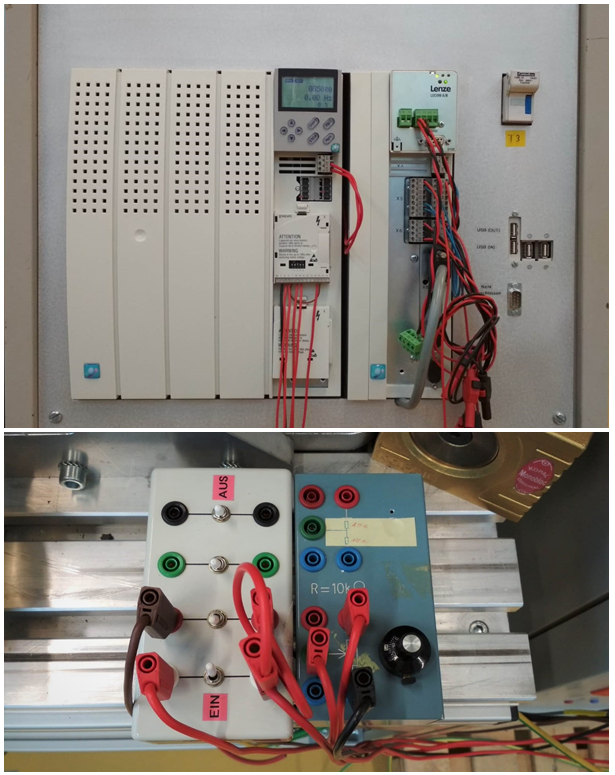
\includegraphics[width=\linewidth]{Versuchsaufbau/SteuerungRegelung.png}
		\caption[Ansteuerung und Regelung]{Ansteuerung und Regelung}
		\label{fig:AnsteuerungRegelung}
	\end{minipage}
\end{figure}

 Die Ansteuerung ist in Abbildung \ref{fig:AnsteuerungRegelung} ersichtlich, wobei die obere Grafik die Steuerungseinheit abbildet. In dieser können verschiedene Ansteuerungsverfahren (Frequenz oder Moment gesteuert) eingestellt werden. Ausserdem können diverse Parameter in der dazugehörigen Code-Tabelle verändert werden, wodurch die ASM optimal angesteuert werden kann. Durch die Veränderung der maximalen Frequenz kann indirekt die Maximaldrehzahl bestimmt werden. Die Frequenz wird durch eine Widerstandsänderung durch ein externes Potentiometer gegeben (Abbildung \ref{fig:AnsteuerungRegelung} unten rechts). Die externe Eingabe kann zudem die Steuerung aktivieren und die Drehrichtung ändern (unten links).

\newpage
\subsection{Drehmoment bei variabler Drehzahl}\label{subsec:DrehmomentDrehzahl}
Um zu beweisen, dass der Motor die erforderliche Leistung erbringt, wird das Drehmoment in Abhängigkeit der Drehzahl untersucht.
Die Bedingungen, mit welchen der Versuch durchgeführt wurde, können der Tabelle \ref{tab:Drehmoment/Drehzahl} entnommen werden.

\begin{table}[H]
\centering
\begin{tabular}{C{4cm} C{4cm} C{3cm}} 
\multicolumn{3}{c}{\textbf{Versuchsbedingungen}} \\
{Messgrösse}& {Bedingung} & {Wert}\\ \hline\hline 
Spannung (DC)   & nachgeregelt &   96 V     \\
Strom (DC)   & gemessen &   37.8-128 A     \\
Leistung (AC)   & gemessen &   1702-8870 W    \\
Drehzahl   & variiert &   614-2954 RPM    \\
Drehmoment-Sollwert   & nachgeregelt &   32 Nm    \\
Motor-Temperatur   & vernachlässigt &   -    \\
Controller-Temperatur   & vernachlässigt &   -    \\
\end{tabular}
\caption{Versuchsbedingungen Drehmoment/Drehzahl-Versuch}\label{tab:Drehmoment/Drehzahl}
\end{table}

Das Drehmoment an der Welle des BLDC-Motors wird mit der Formel \ref{eq:LeistungDrehmoment} in Abhängigkiet zur Leistung und der Drehzahl des Motors ermittelt. Die daraus ermittelte Kurve ist in der Abbildung \ref{fig:drehmoment/drehzahl} (blaue Kurve) ersichtlich. Da die asynchrone Maschine ebenfalls nicht ideal arbeitet und deswegen Verluste aufweist, wird bei dieser ein Wirkungsgrad von 90\% angenommen (rote Kurve).

\begin{equation}
\centering
P = M \cdot \omega = M \cdot 2 \cdot \pi\cdot f
\label{eq:LeistungDrehmoment}
\end{equation}
$P$\quad Leistung		\\
$M$\quad Drehmoment  \\
$\omega$\quad Winkelgeschwindigkeit\\
$f$\quad Frequenz	\\

\begin{figure}[H]
	\centering
	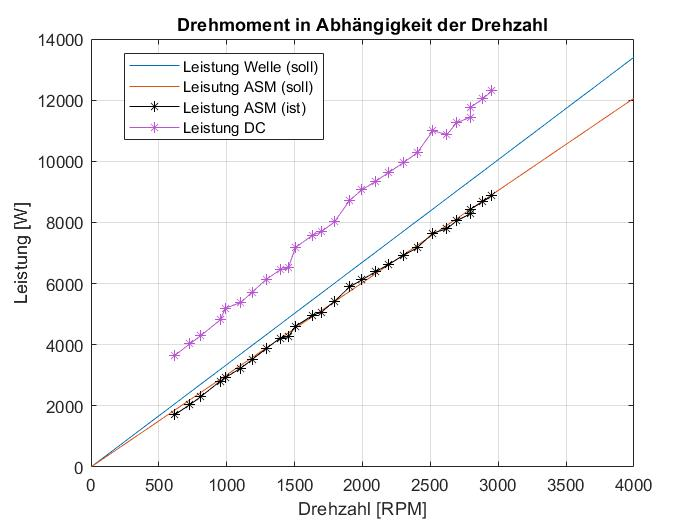
\includegraphics[width=1\linewidth]{drehmoment_drehzahl.jpg}
	\caption{Drehmoment in Abhängigkeit der Drehzahl}\label{fig:drehmoment/drehzahl}
\end{figure}

Bei diesem Versuch ist ersichtlich, dass es möglich ist, die erforderliche Leistung (schwarze Punkte) im Drehzahlbereich zwischen 600 und 3000 RPM (engl. revolutions per minute; \glqq Umdrehungen pro Minute\grqq) zu erreichen. Die aufgenommene Leistung auf der DC-Seite (violette Punkte) ist dabei proportional zur abgegebenen Leistung angestiegen und erreicht bei 3000 RPM einen Wert von über 12kW.

\newpage

In der Abbildung \ref{fig:drehmoment/StromSpannung} sind die Spannung, der Strom und die Sollwertvorgabe für die Ansteuerung während des Versuchs ersichtlich. Die Spannung ist auf $96V_{DC}$ nachgeregelt (blaue Punkte) worden, damit diese für den Versuch konstant bleibt. Der Strom (rote Punkte) und der Sollwert für die Ansteuerung (schwarze Punkte) wurden ebenfalls während des Versuchs dokumentiert.


\begin{figure}[H]
	\centering
	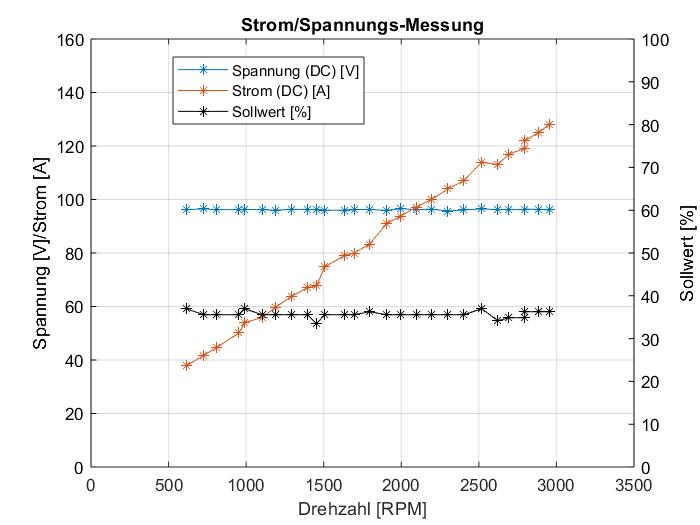
\includegraphics[width=1\linewidth]{drehmoment_StromSpannung.jpg}
	\caption{Spannung und Strom während des Drehmomentversuchs}\label{fig:drehmoment/StromSpannung}
\end{figure}

Der Strom kann mit guter Näherung als linear zur Drehzahl bei gleichbleibendem Drehmoment betrachtet werden. Dadurch ergibt sich bei 3800 RPM ein Strom von ca. 160A, was mit den Werten aus dem Datenblatt des Motors korreliert \cite{MotorData}. Diese maximale Leistung konnte mit diesem Versuchsaufbau jedoch nicht getestet werde, da dieser nur für 11kW ausgelegt ist (Kapitel \ref{subsec:Versuchsaufbau}).

Bei diesem Versuch ist ebenfalls ersichtlich, dass die Sollwertvorgabe über den Drehzahlbereich nur kleine Abweichungen aufweist und daher in guter Näherung als konstant betrachtet werden kann. Die Sollwertvorgabe wurde in Prozent des Minimums (1,2V) und des Maximums (4V) angegeben. Eine genauere Analyse des Sollwertvorgabe ist im Unterkapitel \ref{subsec:Steuerkennlinie} bei der Validierung der Steuerkennlinie ersichtlich.

\subsection{Leistungsabhängigkeit der Temperatur}\label{subsec:Leistung/Temperatur}
Da der BLDC-Motor eine sehr kleine Bauform für seine Leistung hat, unterliegt er grossen Temperaturschwankungen. Deshalb wird untersucht, wie sich die Temperatur bei konstantem Sollwert auf die Leistung auswirkt. Die Versuchsbedingungen können der Tabelle \ref{tab:Leistung/Temperatur} entnommen werden.


\begin{table}[H]
	\centering
	\begin{tabular}{C{4cm} C{4cm} C{3cm}} 
		\multicolumn{3}{c}{\textbf{Versuchsbedingungen}} \\
		{Messgrösse}& {Bedingung} & {Wert}\\ \hline\hline 
		Spannung (DC)   & nachgeregelt &   96 V     \\
		Strom (DC)   & gemessen &   106-112 A     \\
		Leistung (AC)   & gemessen &   7330-7820 W    \\
		Drehzahl   & konstant &   2500 RPM    \\
		Drehmoment-Sollwert   & konstant &   32 Nm    \\
		Motor-Temperatur   & gemessen &   30-100 °C    \\
		Controller-Temperatur   & vernachlässigt &   -    \\
	\end{tabular}
	\caption{Versuchsbedingungen Leistung/Temperatur-Versuch}\label{tab:Leistung/Temperatur}
\end{table}

Wie in der Abbildung \ref{fig:Leistung/Temperatur} ersichtlich ist, nimmt die Leistung bei zunehmender Temperatur ab. Die Leistung verringert sich bei einer Motor-Temperatur von 100°C (gegenüber 30°C) um ca. 6\%. Die Leistungsabnahme ist dabei in guter Näherung linear zur Temperatur.

\begin{figure}[H]
	\centering
	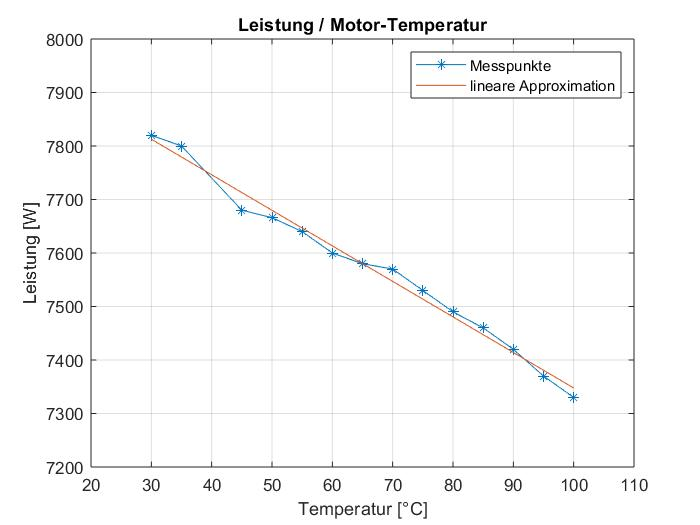
\includegraphics[width=0.9\linewidth]{LeistungTemperatur.jpg}
	\caption{Einfluss der Erwärmung auf die Leistung}\label{fig:Leistung/Temperatur}
\end{figure}

Wird in einem der nachfolgenden Versuche erwähnt, dass die Leistungs-Temperaturabhängigkeit berücksichtigt wurde, ist dies gleichbedeutend mit einer Temperaturskalierung aller Messwerte auf eine Temperatur von 70°C. Dies wird durch Einkalkulierung der in diesem Versuch ermittelte lineare Approximation erreicht, wodurch jeder einzelne Messwert schlussendlich dasselbe Temperaturniveau besitzt und somit die Messung temperaturunabhängig ist.
\subsection{Steuerkennlinie}\label{subsec:Steuerkennlinie}
Die Steuerkennlinie beschreibt die Funktion zwischen dem Input (entspricht einem Regelsignal zwischen 1.2-4V) und dem Drehmoment-Sollwert. Bei diesen Messungen geht es darum, diese Funktion zu bestimmen, um später das angelegte Moment am Motor ohne direkte Kraftmessung regeln zu können. Die Versuchsbedingungen sind in nachfolgender Tabelle \ref{tab:Steuerkennlinie} aufgeführt:

\begin{table}[H]
	\centering
	\begin{tabular}{C{4cm} C{4cm} C{3cm}} 
		\multicolumn{3}{c}{\textbf{Versuchsbedingungen}} \\
		{Messgrösse}& {Bedingung} & {Wert}\\ \hline\hline 
		Spannung (DC)   & nachgeregelt &   96 V     \\
		Strom (DC)   & gemessen &   1.6-107 A     \\
		Leistung (AC)   & gemessen &   0-5666 W    \\
		Drehzahl   & konstant &   1200 RPM    \\
		Drehmoment-Sollwert   & variiert &   0-50 Nm    \\
		Motor-Temperatur   & gemessen &   40-100 °C    \\
		Controller-Temperatur   & vernachlässigt &   -    \\
	\end{tabular}
	\caption{Versuchsbedingungen Steuerkennlinie}\label{tab:Steuerkennlinie}
\end{table}

Wie in der Abbildung \ref{fig:Leistung/Steuerkennlinie} ersichtlich ist, lässt sich das Verhältnis zwischen Drehmoment und Regelsignal mit einer quadratischen Funktion beschreiben. Bei diesem Versuch wird die Leistungs-Temperaturabhängigkeit berücksichtigt, wie sie im Unterkapitel \ref{subsec:Leistung/Temperatur} erklärt wurde.

\begin{figure}[H]
	\centering
	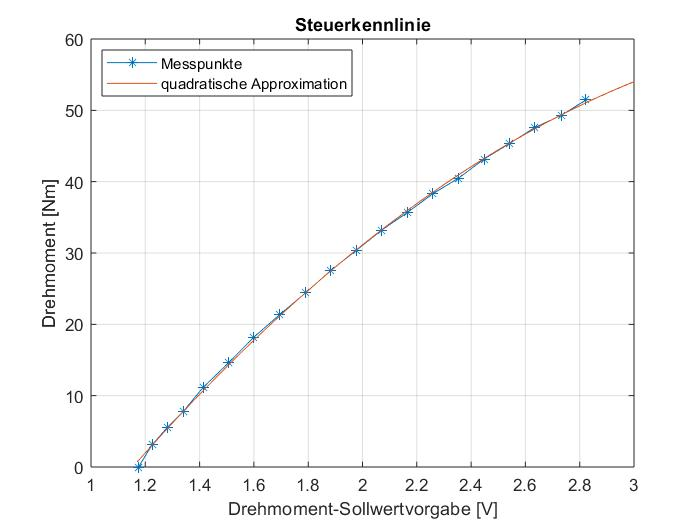
\includegraphics[width=0.9\linewidth]{Steuerkennlinie.jpg}
	\caption{Steuerkennlinie der Ansteuerung}\label{fig:Leistung/Steuerkennlinie}
\end{figure}

Da der Motor bei diesem Versuch an die thermische Grenze kam und für die geplante Anwendung keine höhere Drehmomente erforderlich sind, wird die Messung nur bis 2.8V durchgeführt. Das Maximum des Drehmoment-Sollwertes liegt jedoch bei 4V.
\subsection{Leistungsverhalten bei Spannungsabfall}\label{subsec:LeistungSpannungabfall}
Bei diesem Versuch wird das Verhalten des Controllers bei einem Spannungsabfall untersucht. Dabei wurde sowohl die Leistung der ASM (Abbildung \ref{fig:Spannungsabfall} rechts) als auch der Strom des Controllers (Abbildung \ref{fig:Spannungsabfall} links) in Abhängigkeit zur Spannung des Controllers gemessen. Der Drehmoment-Sollwert wurde während des gesamten Versuchs konstant auf dem Nennmoment gehalten. Die Versuchsbedingungen können der Tabelle \ref{tab:Spannungsabfall} entnommen werden.

\begin{table}[H]
	\centering
	\begin{tabular}{C{4cm} C{4cm} C{3cm}} 
		\multicolumn{3}{c}{\textbf{Versuchsbedingungen}} \\
		{Messgrösse}& {Bedingung} & {Wert}\\ \hline\hline 
		Spannung (DC)   & variiert &   72-103 V     \\
		Strom (DC)   & gemessen &   68.7-124 A     \\
		Leistung (AC)   & gemessen &   4420-6420 W    \\
		Drehzahl   & variiert &   1500/2000 RPM    \\
		Drehmoment-Sollwert   & konstant &   32 Nm    \\
		Motor-Temperatur   & gemessen &   30-90 °C    \\
		Controller-Temperatur   & vernachlässigt &   -    \\
	\end{tabular}
	\caption{Versuchsbedingungen Spannungsabfall}\label{tab:Spannungsabfall}
\end{table}


Auf der Abbildung \ref{fig:Spannungsabfall} sind die Messwerte des Versuchs dargestellt. Zuerst wurde der Versuch mit 2000 RPM (blaue Punkte) und danach nochmals mit 1500 RPM (rote Punkte) durchgeführt. Wird die Leistungs-Temperaturabhängigkeit berücksichtigt (schwarze und rosa Punkte), dann ist ersichtlich, dass die Leistung nicht von der Spannung, sondern lediglich von der Temperatur abhängig ist.

\begin{figure}[H]
	\centering
	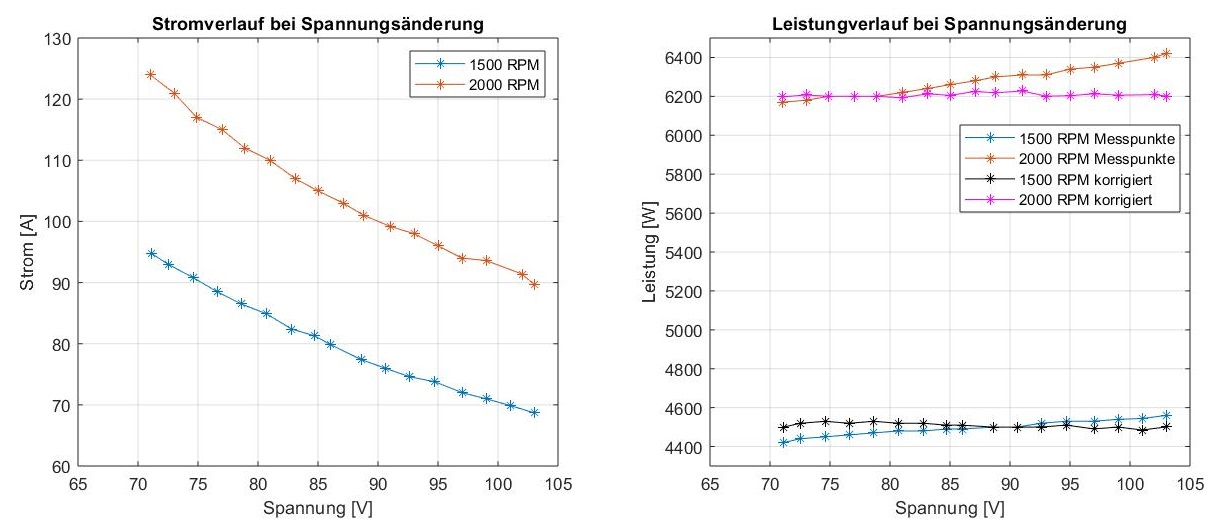
\includegraphics[width=1\linewidth]{Spannungsversuch.jpg}
	\caption{Leistungs- und Stromverlauf bei Spannungsabfall}\label{fig:Spannungsabfall}
\end{figure}

\subsection{Temperatur}\label{subsec:Temperatur}
Um einen Einblick in das Temperaturverhalten des Motors zu erlangen, wurde in diesem Versuch die Erwärmung in Abhängigkeit der Drehzahl bei konstantem Moment gemessen. Die Messung erfolgte bei einer Drehzahl von 1550 RPM und bei 2550 RPM, und einem jeweiligen Drehmoment von 32Nm. Die Starttemperatur des Motors lag jeweils bei ca. 60°C und wurde solang betrieben, bis er eine Betriebstemperatur von 100°C erreicht hatte.


\begin{figure}[H]
	\centering
	\includegraphics[width=0.8\linewidth]{Temperatur.jpg}
	\caption{Erwärmung}\label{fig:Temperatur}
\end{figure}


Da die Leistung sowohl vom Drehmoment als auch von der Drehzahl abhängig ist, wurde beim Versuch bei 2550RPM eine höhere Leistung und somit auch ein grösseren Strom erzielt. Aus diesem Grund ist die Erwärmung des Motors bei höheren Drehzahlen dementsprechend grösser. Anhand der beiden Versuchen gehen wir davon aus, dass der BLDC-Motor ca. 5 Minuten unter Vollast betrieben werden kann, bis er die 100°C erreicht. Es gilt zu beachten, dass der Motor eine Betriebstemperatur von 110°C zulässt, wodurch eine Reserve von 10°C gegeben ist.
\subsection{Maximale Leistung bei variabler Spannung}\label{subsec:LeistungSpannungsabfall}
In diesem Versuch wird die maximale Leistung bei einem Spannungsabfall untersucht. Da die asynchrone Maschine nicht für 3800 RPM ausgelegt ist, wurde dieser Versuch bei einer konstanten Drehzahl von 3600 RPM gemessen. Wie im vorhergehenden Versuch, wurde das Drehmoment aufs Maximum eingestellt, während die Spannung langsam erhöht wurde.


\begin{figure}[H]
	\centering
	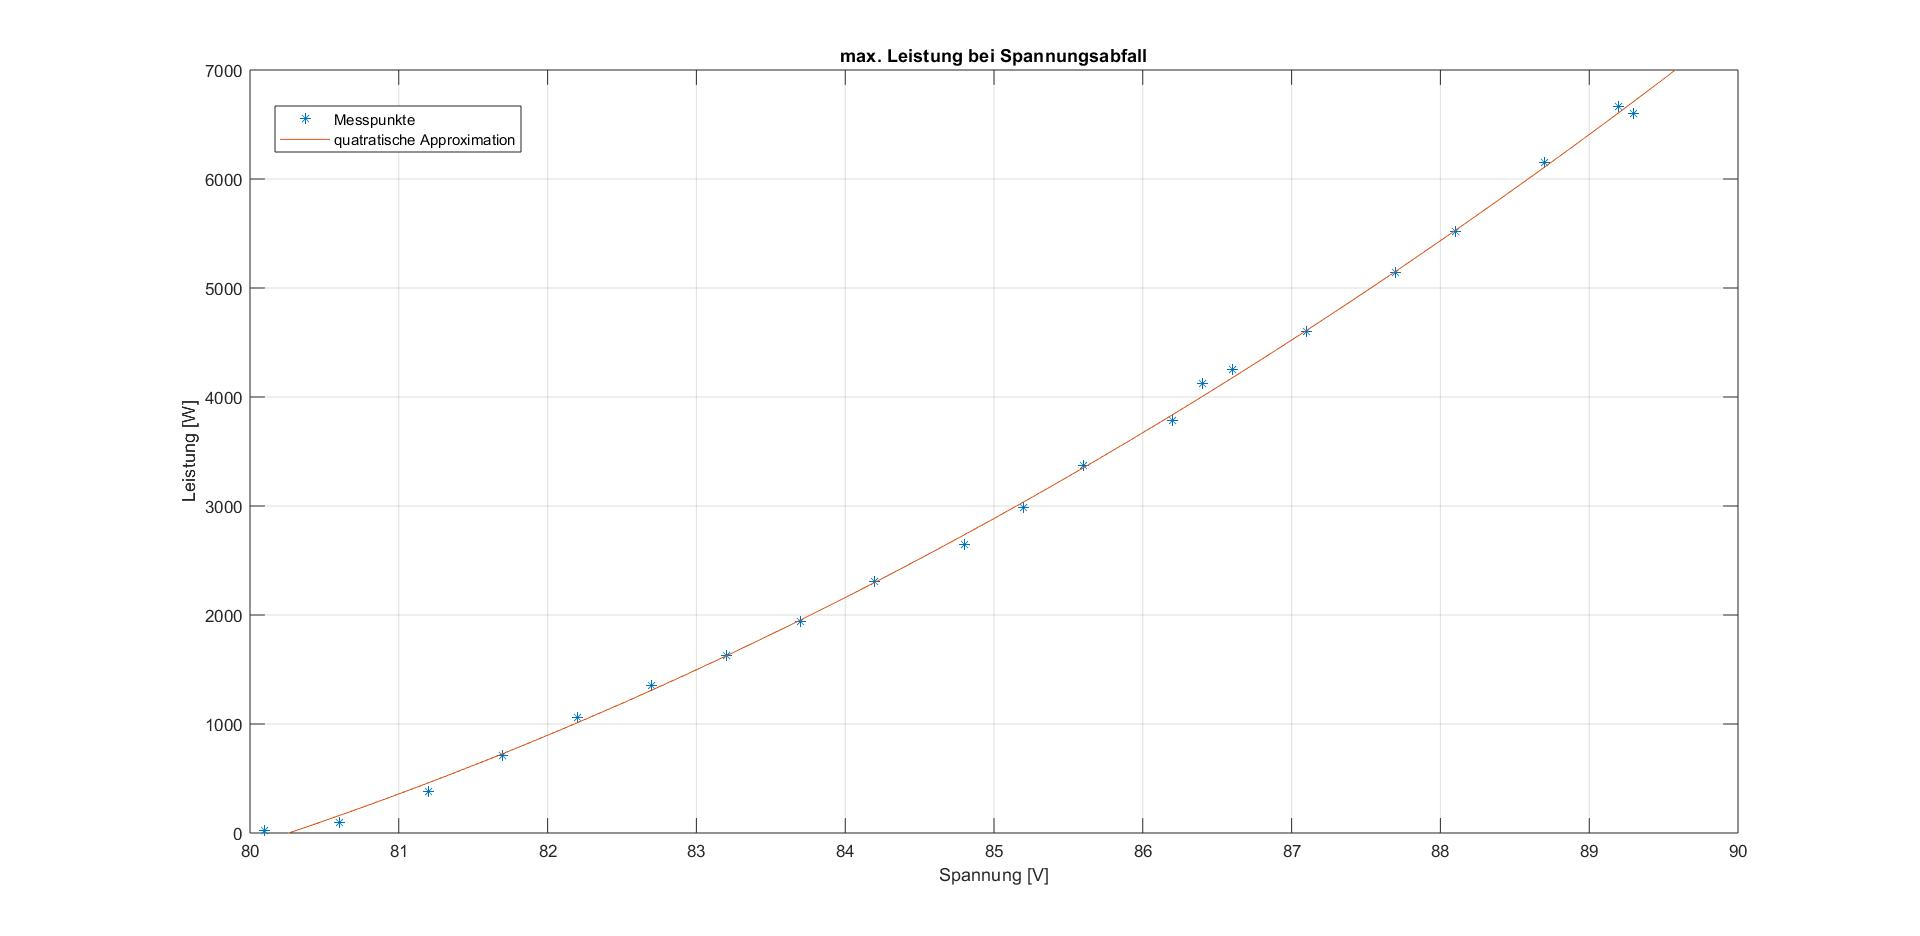
\includegraphics[width=0.8\linewidth]{maxLeistung.jpg}
	\caption{Maximale Leistung}\label{fig:maxLeistung}
\end{figure}

Unter der Annahme, dass zwischen der maximalen Leistung und der Spannung ein quadratischer Zusammenhang besteht (rote Approximation), ist anzunehmen, dass die maximale Leistung bei 3600 RPM und Nennspannung (96V) bei 15kW liegt. Hierbei ist jedoch anzumerken, dass die effektive Leistung an der Welle des BLDC-Motors ca. 10\% höher ist, da diese auf der elektrischen Seite der asynchronen Maschine gemessen wurde.
 
\subsection{Maximale Drehzahl bei variabler Spannung}\label{subsec:DrehzahlSpanungsabfall}
In diesem Versuch wird das Verhalten des Motors bei Unterspannung untersucht. Dabei wird der Sollwert für das Drehmoment auf dem Maximum gehalten, während der Motor im Leerlauf dreht. Die Spannung wird dabei langsam erhöht.

\begin{table}[H]
	\centering
	\begin{tabular}{C{4cm} C{4cm} C{3cm}} 
		\multicolumn{3}{c}{\textbf{Versuchsbedingungen}} \\
		{Messgrösse}& {Bedingung} & {Wert}\\ \hline\hline 
		Spannung (DC)   & variiert &   64.7-90.7 V     \\
		Strom (DC)   & gemessen &   9.33-13.1 A     \\
		Leistung (AC)   & vernachlässigt &   -    \\
		Drehzahl   & gemessen &   3600 RPM    \\
		Drehmoment-Sollwert   & konstant &   max.    \\
		Motor-Temperatur   & vernachlässigt &   -    \\
		Controller-Temperatur   & vernachlässigt &   -    \\
	\end{tabular}
	\caption{Versuchsbedingungen max. Drehzahl}\label{tab:maxDrehzahl}
\end{table}

Damit der Motor nicht durch zu hohe Drehzahlen beschädigt wird, kann beim Controller eine Drehzahlobergrenze eingestellt werden. Diese ist für diesen Versuch auf 3800 RPM begrenzt, weil die asynchrone Maschine keine höheren Drehzahlen zulässt. Die maximale Drehzahl ist in nachfolgender Abbildung \ref{fig:maxDrehzahl} graphisch dargestellt.

\begin{figure}[H]
	\centering
	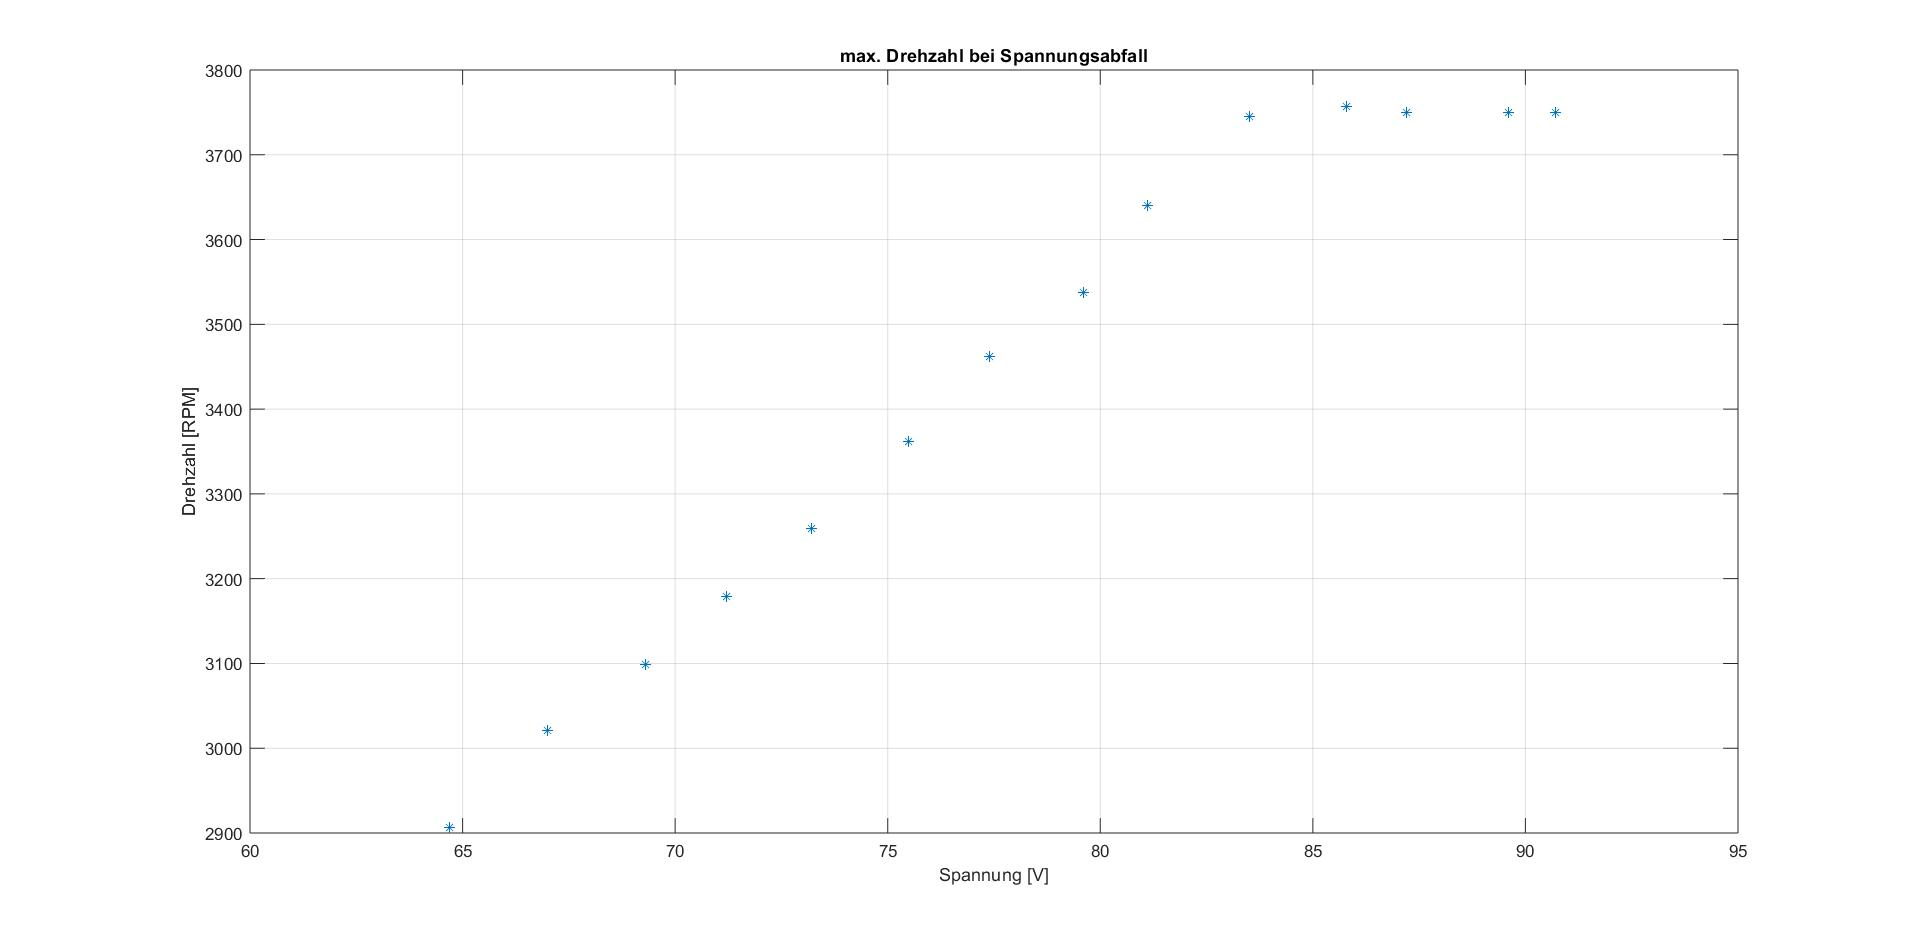
\includegraphics[width=0.8\linewidth]{maxDrehzahl.jpg}
	\caption{Maximale Drehzahl im Leerlauf}\label{fig:maxDrehzahl}
\end{figure}


Bei diesem Versuch hat sich gezeigt, dass die DC-Spannung mindestens 84V betragen muss, damit der BLDC-Motor in Feldschwächung kommt und somit eine Drehzahl von 3800 RPM erreichen kann. Weiter ist ersichtlich, dass die Leerlaufdrehzahl ca. 45 RPM pro Volt sinkt.
\subsection{Quantitative Versuche}\label{subsec:Quantitative}
In diesem Versuch werden kurz die Versuche und deren Erkenntnis erläutert, bei welchen die Ergebnisse nicht qualitativ ermittelt werden konnten.
\begin{itemize}
	\item \textbf{Welligkeit:} Da die Welligkeit der Zugkraft maximal $\pm$25N betragen darf (Anhang \ref{appsec:Anforderungen} Punkt 01-03), wurde das Verhalten bei Änderung der Drehzahl und der Leistung beobachtet. Dabei konnten keine Kraftschwankungen auf dem System wahrgenommen oder gemessen werden.
	\item \textbf{Lastabwurf:} Um festzustellen, wie das System bei einem plötzlichen Lastabwurf reagiert, wurde dieser ebenfalls simuliert. Dabei hat sich gezeigt, dass die Drehzahl kurzzeitig stark ansteigt (auch über die Drehzahlbegrenzung), die Ansteuerung danach jedoch innerhalb von wenigen Sekunden auf die Drehzahl des Maximums zurückregelt.
\end{itemize}
\subsection{Fazit}\label{subsec:Fazit}
In diesem Unterkapitel werden die Erkenntnisse der Versuche kurz zusammengefasst.\\

Bei den Spannungsversuche hat sich gezeigt, dass die Versorgungsspannung in einem grossen Bereich keinen Einfluss auf die Ansteuerung hat. Bei hohen Leistungen hat sich jedoch gezeigt, das eine zu geringe Spannung zu einem Leistungsabfall führt. Werden die Resultate aus den Versuchen \glqq Maximale Drehzahl bei variabler Spannung\grqq (\ref{subsec:DrehzahlSpanungsabfall}) und \glqq Maximale Leistung bei variabler Spannung\grqq (\ref{subsec:LeistungSpannungsabfall}) berücksichtigt, dann ist ersichtlich, dass die Leistung nur erbracht werden kann, wenn die Nennspannung (96V) am System anliegt. Da die Batteriespannung bei hohen Ströme leicht einbricht (Unterkapitel \ref{subsec:Energieversorgung}), wird bei hohen Leistung eine Kraftreduzierung erwartet. In der Abbildung \ref{fig:LeistungKraft} ist die Leistung und die Kraft bezogen auf die Geschwindigkeit aufgezeigt. Im unteren Geschwindigkeitsbereich ist die Leistung proportional zur Geschwindigkeit, da die Kraft konstant gehalten wird. Im oberen Bereich wird die Leistung durch die Spannung begrenzt, wodurch die Kraft linear zur Geschwindigkeit abnimmt.

\begin{figure}[H]
	\centering
	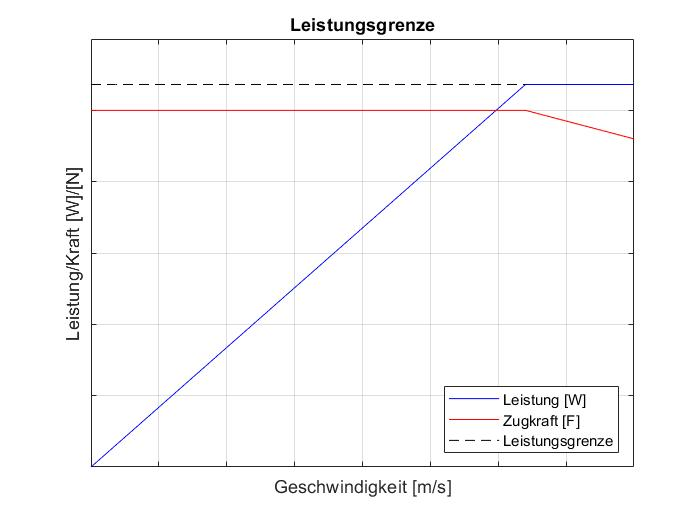
\includegraphics[width=1\linewidth]{LeistungKraft.jpg}
	\caption{Leistungsgrenze}\label{fig:LeistungKraft}
\end{figure}

Diese Leistungsgrenze ist abhängig von der Energieversorgung. Da diese mit Batterien realisiert wird, ist der Innenwiderstand der Batterie ein wichtiger Faktor. Zudem hat der Ladezustand einen Einfluss darauf, da die Spannung der Batterie beim entladen dieser abnimmt.\\
Bei einer stabilen Spannungsquelle war anhand des Drehmoment/Leistungs-Versuch ersichtlich, dass der Motor die erforderliche Leistung erbringen kann und dass die Kraftregelung der Ansteuerung genügend präzise für die geplante Anwendung ist. Einzig im Leerlauf bei geringen Drehzahlen ist die Geschwindigkeitsregelung schwierig.\\
Die Temperatur-Versuche haben zudem aufgezeigt, dass sowohl der Motor als auch die Ansteuerung gekühlt werden müssen, da diese sonst überhitzen. Vor allem im Abrollbetrieb, wenn ein höherer Intervall erreicht werden kann, muss der Motor gut gekühlt werden.\\
Anhand der Versuche konnte bewiesen werden, dass der Motor alle Anforderungen für den Einzugsbetrieb erfüllt. Die effektive maximale Leistung hängt jedoch von der Energieversorgung ab. Da diese wiederum vom Innenwiderstand, Batterietyp und dem Ladezustand abhängt, kann eine definitive Aussage über die max. Leistung erst am definitiven Ausbau gemacht werden.
